\section{Реализация}
\subsection{Модель}
Для начала определим, какие классы необходимо добавить в систему.  Для хранения информации о альбомах добавим новый класс \textbf{Album}  с атрибутами: имя альбома (string), id альбома (integer), id персоны (integer), id фильма (integer). Однако при этом возникает несколько проблем:

\begin{itemize}
\item Поиск по идентификатору происходит намного быстрее, чем поиск на сравнение двух строк.
\item Хранить для каждого фильма отдельный альбом в виде строки не оптимально, это лишняя нагрузка на БД.
\end{itemize}

Избежать всего этого можно, выделив фотографии в отдельный класс. В результате мы получим:

\begin{figure}[h!]
\begin{center}
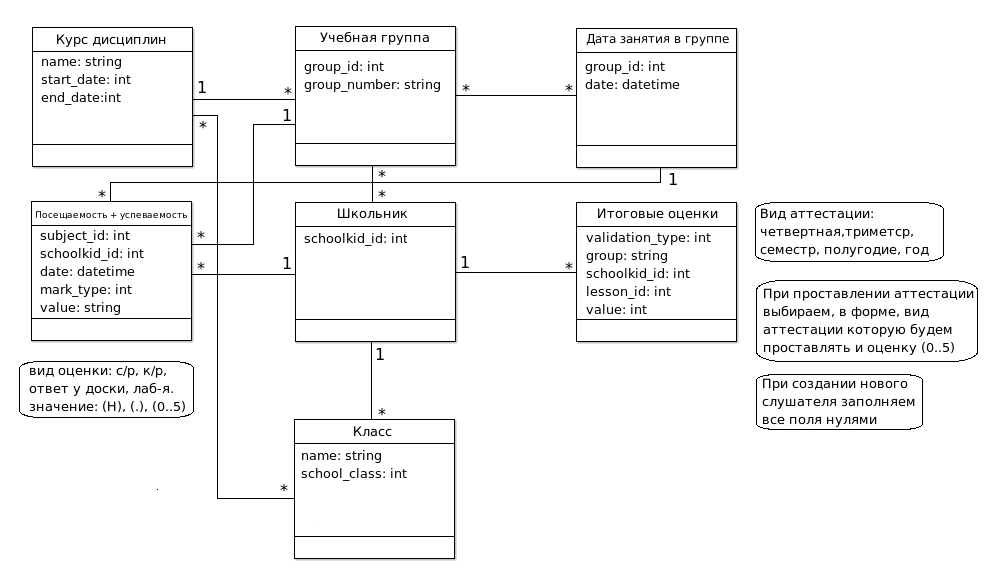
\includegraphics[scale=0.9]{image/class_my.png}
\end{center}
\caption{Диаграмма классов: индивидуальная часть}
\end{figure}

Из диаграммы видно, что теперь класс \textbf{Album} содержит id персон, фильмов и альбомов. Он связан отношением многие ко многим с классом \textbf{Image} (фотография), \textbf{Films} (фильмы) и \textbf{Persons} (персоны). Класс \textbf{Image} хранит информацию о фотографиях: К какому альбому принадлежит фотография(связь через id альбома), какой тип имеет(фоторафия или скриншот). Теперь, после определения классов и их атрибутов, которые будут в нашей системе, можно переходить к реализации.\\
Так как для каждого класса необходимы модель, контроллер и представления воспользуемся генератором \textit{scaffold}, и сгенерируем все части с его помощью.
\verbatiminput{code/sc.txt}
Внесем изменения в модель \textbf{Images:}
\verbatiminput{code/image_modt.txt}
Здесь указана связь многие ко многим с классом \textbf{Album} (belongs\_to \:album). Также добавлены ограничения: id альбома должен быть всегда не пустым. 
А также добавим изменения в главную модель: \textbf{Album:}. 

\verbatiminput{code/album_mod.txt}
Вначале указаны связи с классами \textbf{Image} (has\_many \:images), \textbf{Persons} (belongs\_to \:person), \textbf{Films} (belongs\_to \:film) и \textbf{User} (belngs\_to \:user). Также добавлены несколько проверок на корректность вводимых пользователем данных: имя альбома не может быть пустым, оно уникально и имеет длину от 3 до 40 символов. Также определена интересная валидация, используемая для того чтобы при создании альбома нельзя было привязать его сразу к персоне и фильму, либо сразу ни к персоне ни к фильму. Далее определены несколько методов, которые понадобятся в дальнейшем. Для удобного просмотра фотографий сделаем удобную навигацию с помощью плагина fancy_box, с возможнотью пролистывания фотографий или автоматического слайдшоу.\\

В моделях классов \textbf{Person} и \textbf{Films} также необходимо указать связи с классом \textbf{Album}.

\verbatiminput{code/p_f_mod.txt}

\subsection{Контроллер и Представление}
Теперь, после внесения всех необходимых изменений в модели, можно переходить к контроллерам. Контроллер интерпретирует данные, введённые пользователем, и информирует модель и представление о необходимости соответствующей реакции.\\
\hspace*{0.25cm}Для того чтобы пользователь мог добавлять альбомы, не нужно создавать отдельный интерфейс, можно сделать это при редактировании персоны или фильма. Для этого просто добавим ссылку на страничку создания альбома. 
Рассмотрим, как это будет выглядеть для класса \textbf{Album}.

\verbatiminput{code/form.txt}

Необходимо добавить небольшой скрипт, который будет посылать запрос в фоновом режиме к контролеру и ожидать результатов поиска. При этом контролер может извлекать данные из любого места, как, например, базы данных или жесткого диска. Но результаты поиска должны возвращаться  в формате \textit{JSON}.

\verbatiminput{code/js.txt}

Также необходимо добавить создание, отображение, редактирование, удаление, изменени и сохранение нового альбома в контроллере альбома.

\verbatiminput{code/update.txt} 

Вначале находится персона, у которой \textit{id} равен \textit{params[:id]}, этот параметр передается от формы при ее редактировании. После этого создаётся новый альбом и сохраняется. Если пользователь не ввел никакой информации, то альбом не сохраняется. Если не удалось сохранить альбом (а это возможно только в одном случае -- данные, введенные пользователем,  не прошли проверку), делается возврат в форму, и отображается сообщение об ошибке пользователю.\\
\hspace*{0.5cm}Для того чтобы сделать возможным просмотр всех альбомов у персоны или фильма, нужно внести изменения в представление персоны или фильма, а именно в метод 
\textit{show}.
\verbatiminput{code/show_person.txt}

Аналогичным образом реализуется просмотр альбома у фильма.
\verbatiminput{code/film_prize.txt}

\endinput

